%%%%%%%%%%%%%%%%%%%%%%%%%%%%%%%%%%%%%%%%%
% Masters/Doctoral Thesis 
% LaTeX Template
% Version 2.3 (25/3/16)
%
% This template has been downloaded from:
% http://www.LaTeXTemplates.comx
%
% Version 2.x major modifications by:
% Vel (vel@latextemplates.com)
% Minor modifications (unversioned) by bong0 (https://github.com/bong0)
%
% This template is based on a template by:
% Steve Gunn (http://users.ecs.soton.ac.uk/srg/softwaretools/document/templates/)
% Sunil Patel (http://www.sunilpatel.co.uk/thesis-template/)
%
% Template license:
% CC BY-NC-SA 3.0 (http://creativecommons.org/licenses/by-nc-sa/3.0/)
%
%%%%%%%%%%%%%%%%%%%%%%%%%%%%%%%%%%%%%%%%%

%----------------------------------------------------------------------------------------
%	PACKAGES AND OTHER DOCUMENT CONFIGURATIONS
%----------------------------------------------------------------------------------------

\documentclass[
12pt, % The default document font size, options: 10pt, 11pt, 12pt
oneside, % Two side (alternating margins) for binding by default, uncomment to switch to one side
chapterinoneline,% Have the chapter title next to the number in one single line
ngerman, % ngerman for German
onehalfspacing, % Single line spacing, alternatives: onehalfspacing or doublespacing
draft=false, % Uncomment to enable draft mode (no pictures, no links, overfull hboxes indicated)
nolistspacing, % If the document is onehalfspacing or doublespacing, uncomment this to set spacing in lists to single
%liststotoc, % Uncomment to add the list of figures/tables/etc to the table of contents
%toctotoc, % Uncomment to add the main table of contents to the table of contents
%parskip, % Uncomment to add space between paragraphs
%nohyperref, % Uncomment to not load the hyperref package
headsepline % Uncomment to get a line under the header
%printmode % turns on and off coloring of links
%openany % disables strict start of any listing/chapter on odd page and therefore empty pages padding
]{MastersDoctoralThesis} % The class file specifying the document structure

\usepackage[utf8]{inputenc} % Required for inputting international characters
\usepackage[T1]{fontenc} % Output font encoding for international characters

%\usepackage{palatino} % Use the Palatino font by default
\usepackage{lmodern}


\usepackage{blindtext}

%----------------------------------------------------------------------------------------
%	MARGIN SETTINGS
%----------------------------------------------------------------------------------------

\geometry{
	paper=a4paper, % Change to letterpaper for US letter
	inner=2.5cm, % Inner margin
	outer=3.8cm, % Outer margin
	bindingoffset=2cm, % Binding offset
	top=1.5cm, % Top margin
	bottom=1.5cm, % Bottom margin
	%showframe,% show how the type block is set on the page
}


\newcommand{\raisedrule}[2][0em]{\leaders\hbox{\rule[#1]{1pt}{#2}}\hfill}

%----------------------------------------------------------------------------------------
%	THESIS INFORMATION
%----------------------------------------------------------------------------------------

%%
% Buzzwordsammlung
% Privatsphäre, Überwachung, Ende-zu-Ende E-Mail Verschlüsselung, sicher, PKI, 
% Automatisierung, datensparsam
%%
\thesistitle{Ein Beispieltitel für eine Thesis der mehrere Zeilen umfasst und seriös wirkt} % Your thesis title, this is used in the title and abstract, print it elsewhere with \ttitle
\supervisor{Prof. Dr. Max Mustermann} % Your supervisor's name, this is used in the title page, print it elsewhere with \supname
\examiner{Prof. Dr. Jane Example} % Your examiner's name, this is not currently used anywhere in the template, print it elsewhere with \examname
\degree{Bachelor of Science (B.Sc.)} % Your degree name, this is used in the title page and abstract, print it elsewhere with \degreename
\author{John Doe} % Your name, this is used in the title page and abstract, print it elsewhere with \authorname
\addresses{} % Your address, this is not currently used anywhere in the template, print it elsewhere with \addressname

\subject{Informatik} % Your subject area, this is not currently used anywhere in the template, print it elsewhere with \subjectname
\keywords{Buzzword1;Buzzword2;RFC9999} % Keywords for your thesis, this is not currently used anywhere in the template, print it elsewhere with \keywordnames
\university{\href{https://www.h-da.de}{Hochschule Darmstadt}} % Your university's name and URL, this is used in the title page and abstract, print it elsewhere with \univname
%\department{\href{http://department.university.com}{Department or School Name}} % Your department's name and URL, this is used in the title page and abstract, print it elsewhere with \deptname
%\group{\href{http://researchgroup.university.com}{Research Group Name}} % Your research group's name and URL, this is used in the title page, print it elsewhere with \groupname
\faculty{\href{https://fbi.h-da.de}{Fachbereich Informatik}} % Your faculty's name and URL, this is used in the title page and abstract, print it elsewhere with \facname



\newif\ifkoma

%\usepackage[german]{fancyref} not used atm


\makeatletter
\@ifclassloaded{scrartcl}{\komatrue}{\komafalse}
\makeatother

\usepackage[usenames,dvipsnames,svgnames,table]{xcolor}

% Das wird in neueren Versionen von Pandoc benutzt:
\providecommand{\tightlist}{%
  \setlength{\itemsep}{0pt}\setlength{\parskip}{0pt}}

% Stellt \euro zur Verfügung:
\usepackage{eurosym} 

\usepackage{amssymb,amsmath}
\usepackage{ifxetex,ifluatex}
\ifxetex
  \usepackage{fontspec,xltxtra,xunicode}
  \defaultfontfeatures{Mapping=tex-text,Scale=MatchLowercase}
\else
  \ifluatex
    \usepackage{fontspec}
    \defaultfontfeatures{Mapping=tex-text,Scale=MatchLowercase}
    % Die 6 Vista-Fonts:
    %   1. Calibri:       Serifenlos, Ersatz für Verdana (war Ersatz für Arial)
    %   2. Cambria:       Ersatz für Times New Roman
    %   3. Candara:       (für informelle Schriftstücke)
    %   4. Consolas:      Nicht-Proportional-Schrift für Quelltexte
    %   5. Constantia:    Für Fließtexte für Print- und elektronische Medien
    %   6. Corbel:        Serifenlos, für die Bildschirmdarstellung, enthält Mediävalziffern
    \setsansfont{Calibri}
    \setromanfont{Cambria}
    %\setromanfont{Constantia}
    \setmonofont{Consolas}
  \else
    \usepackage[utf8]{inputenc}
    % UTF-8-Zeichen, die direkt im TeX-Quelltext stehen dürfen
    % --------------------------------------------------------
    % Doppelte Dollar-Zeichen für die math-Umgebung sind notwendig, wegen des
    % Pandoc-Expansionsmechanismus für Variablen.
    % Die Liste der Unicode-Zeichen, die über die Tastatur erreichbar sind,
    % findet man hier: 
    %   <url:/usr/share/X11/locale/en_US.UTF-8/Compose>
    % Der Compose-Key (= Multi_Key) ist ROLLEN (bei mh, einstellbar über
    % KDE-Einsgtellungen). 
    % Man drückt den Compose-Key, lässt ihn los und tippt dann zwei weitere
    % Zeichen ein.
    
    % €  Unicode Character 'EURO SIGN' (U+20AC), UTF-8 = E2 82 AC 
    % <url:http://www.fileformat.info/info/unicode/char/20aC/index.htm>
    \DeclareUnicodeCharacter{20AC}{\euro}

    % €  Unicode Character 'SECTION SIGN' (U+00A7), UTF-8 = c2 a7 (Paragraphenzeichen)
    \DeclareUnicodeCharacter{C2A7}{\S}

    % ←  Unicode Character 'LEFTWARDS ARROW' (U+2190),UTF-8 = E2 86 90, Compose< -  
    % vgl. <url:http://www.fileformat.info/info/unicode/char/2190/index.htm>
    \DeclareUnicodeCharacter{2190}{\mbox{$\leftarrow$}}

    % →  Unicode Character 'RIGHTWARDS ARROW' (U+2192), UTF-8 = E2 86 92, Compose- >:
    % (Das Zeichen wird in einigen Fonts wie ein Minus-Zeichen dargestellt. Das
    % ist ein Fehler im Font, der Zeichencode wird korrekt gebildet.)
    % vgl. <url:http://www.fileformat.info/info/unicode/char/2192/index.htm>
    \DeclareUnicodeCharacter{2192}{\mbox{$\rightarrow$}}

    %\usepackage{pxfonts}       % Palatino-likes fonts for TeX (breiter)
    %\usepackage{txfonts}        % Times-likes font for TeX (schmaler als Palatino) Julian disabled
    %\usepackage{lmodern}       % latin modern fonts
  \fi
\fi


\ifkoma
	%% Das ist ungetestet (2015-08-15):
	% Das ist der Font für "Abbildung 2":
	\addtokomafont{captionlabel}{\bfseries\small}
	% Das ist der Font für die eigentliche Beschreibung:
	\addtokomafont{caption}{\itshape\small}
	% Beschreibung nicht hängend unter Label setzen:
	\setcapindent{0em}
	% Das erzeugt »Abbildung 2.«, anstelle von »Abbildung 2:«.
	\renewcommand*{\captionformat}{.\ }
\fi

% if(tables)
\usepackage{ctable}
\usepackage{float} % provides the H option for float placement
% end(tables)

% if(url)
\usepackage[hyphens]{url}
% end(url)

%Funktioniert nicht gut:
% \renewcommand{\texttt}[1]{\color{red}#1\color{black}}

% Hier kommt z.B. Code von Pygments (automatisch):


 %%%%%%%%%%%%%%%%%%%%%%%%%%%%%%%%%%%%%%%%%%%%%%%
% Additions 
% define fbox border (for framing images e.g.)
\setlength\fboxrule{0.5pt}

\usepackage{subcaption}
\usepackage{float}
%\usepackage{subfig}

\makeatletter
\def\figcaption{%
	\refstepcounter{figure}%
	\@dblarg{\@caption{figure}}}
\makeatother


%\pagestyle{scrheadings}
%\usepackage[pdfspacing]{classicthesis}

\usepackage{enumitem}

%\clearscrheadfoot
%\ohead{\rightmark}
%\cfoot[\pagemark]{\pagemark}

\usepackage{translator} % macht aus "Acronyms" Akronyme
\deftranslation[to=German]{Acronyms}{Akronyme}

%Glossar, Abkürzungsverzeichnis, Symbolverzeichnis
\usepackage[nonumberlist, acronym, nomain, style=long]{glossaries}
%Glossar-Befehle anschalten
\makeglossaries
\renewcommand{\glsnamefont}[1]{\textbf{#1}}
	
%Diese Befehle sortieren die Einträge in den
%einzelnen Listen:
%makeindex -s datei.ist -t datei.alg -o datei.acr datei.acn
%makeindex -s datei.ist -t datei.glg -o datei.gls datei.glo
%makeindex -s datei.ist -t datei.slg -o datei.syi datei.syg

\newcommand*{\myglossaryindent}{0cm}

\newglossarystyle{longwithindent}{%
	\glossarystyle{long}%
	\renewenvironment{theglossary}%
	{\begin{longtable}[l]{@{\hspace{\myglossaryindent}}lp{\glsdescwidth}lp{\glspagelistwidth}@{}}}%
		{\end{longtable}}%
} 

\newacronym{RFC}{RFC}{Request for Comments}
\newacronym{CA}{CA}{Certification Authority}
\newacronym{RA}{RA}{Registration Authority}
\newacronym{VV}{VV}{Volksverschlüsselung}
\newacronym{PKI}{PKI}{Public Key Infrastructure}
\newacronym[plural={CRLs}, firstplural=Certificate Revocation Lists]{CRL}{CRL}{Certificate Revocation List}
%\acrodefplural{CRL}[CRLs]{Certificate Revocation Lists}
\newacronym{API}{API}{Application Programming Interface}
\newacronym{BC}{BC}{BouncyCastle}
\newacronym{UID}{UID}{User ID}
%\newacronym{UTF8}{UTF-8}{UTF-8 Zeichenkodierung}
\newacronym{SFTP}{SFTP}{Secure File Transfer Protocol}
\newacronym{HSM}{HSM}{Hardware Security Module}
\newacronym{JCA}{JCA}{Java Cryptography Architecture}
\newacronym{JCE}{JCE}{Java Cryptography Extension}
\newacronym{BLOB}{BLOB}{Binary Large Object}
\newacronym{PGP}{PGP}{Pretty Good Privacy}
\newacronym{GPG}{GPG}{GNU Privacy Guard}
\newacronym{WoT}{WoT}{Web of Trust}
\newacronym{E2E}{E2E}{Ende-zu-Ende}
\newacronym{OT}{OT}{Owner-Trust}
\newacronym{bnetza}{BNetzA}{Bundesnetzagentur}
\newacronym{IETF}{IETF}{Internet Engineering Task Force}
\newacronym{GPL}{GPL}{GNU Public License}
\newacronym{UTC}{UTC}{Coordinated Universal Time}
\newacronym{svn}{svn}{Subversion}
\newacronym{ECC}{ECC}{Elliptic-Curve-Cryptography}
\newacronym{BSI}{BSI}{Bundesamt für Sicherheit in der Informationstechnik}
\newacronym{CSP}{CSP}{Certification Service Provider}
\newacronym{PKC}{PKC}{Public Key Kryptographie}
\newacronym{ID}{ID}{Identifikationsnummer}
\newacronym{CMP}{CMP}{Certificate Management Protocol}
\newacronym[shortplural={GZHK},longplural={Größten Zusammenhangskomponente}]{GZHK}{GZHK}{Größte Zusammenhangskomponente}
\newacronym{JSON}{JSON}{Javascript Object Notation}
\newacronym{NIST}{NIST}{National Institute of Standards and Technology}
\newacronym{ER}{ER}{Entity-Relationship}
\newacronym{BNetzA}{BNetzA}{Bundesnetzagentur}



%\usepackage[square,sort,comma,numbers]{natbib}

\usepackage[backend=biber,style=alphabetic,natbib=true]{biblatex} % Use the bibtex backend with the authoryear citation style (which resembles APA)
\DefineBibliographyStrings{ngerman}{%
	urlseen={zuletzt besucht am:}% %%% not `visited on'
}
\setcounter{biburllcpenalty}{1000} % Zeilenumbrüche in Url bei jedem belibigen Buchstaben 

\usepackage[nameinlink]{cleveref}
\usepackage{nameref}

% Store \vref in a variable to enable redefining itself.
% Redefine \vref so the hyperlink is extended to the entire
% reference.
\let\vrefpointer\vref
\renewcommand{\vref}[1]{%
	\hyperref[#1]{\vrefpointer{#1}}%
}

% A custom command \smartref with the hyperlink extended to 
% the entire reference. 
% Plus some grammatic sugar (quote marks and comma)
\newcommand{\smartref}[1]{%
	\hyperref[#1]{\cref{#1}, \glqq\nameref{#1}\grqq, \vpageref{#1}}%
}

% define cref listings since its version is too old
\crefname{lstlisting}{}{} % if you fill "listing" and "listings" in there the noun will be doubled, to clear it...
\Crefname{lstlisting}{Listing}{Listings}

%%% fullref is evil! pages off, use vref

%fix for bug in biblatex http://tex.stackexchange.com/a/311428
\makeatletter
\def\blx@maxline{77}
\makeatother

\usepackage[autostyle]{csquotes}  

%Quellcode
\usepackage{listingsutf8}

%\usepackage[round, sort, compress, authoryear]{natbib}

%\usepackage[%
%style=ieee,%
%%   style=numeric,
%isbn=true,%
%doi=false,%
%sorting=none,%
%url=true,%
%defernumbers=true,%
%bibencoding=utf8,%
%backend=biber%
%]{biblatex}

%Den Punkt am Ende jeder Beschreibung deaktivieren
\renewcommand*{\glspostdescription}{}

%%%%%%%%%%%%%%%%%%%% Quelltext Element - Style-File %%%%%%%%%%%%%%%%%%%%%%%
\usepackage[varqu]{zi4}
\definecolor{eclipse-red}{RGB}{127,0,85}
\definecolor{eclipse-blue}{RGB}{0,0,192} %for fields
\definecolor{eclipse-strings}{RGB}{42,0,255}
\definecolor{eclipse-green}{RGB}{63,127,95}
\definecolor{eclipse-lightblue}{RGB}{127,159,191} %for Javadoc Tags
\definecolor{eclipse-gray}{RGB}{100,100,100} %for annotations
\definecolor{eclipse-JavadocHTML}{RGB}{127,127,159} %for Javadoc HTML
\definecolor{eclipse-JavadocLinks}{RGB}{63,63,191}
\definecolor{eclipse-Javadoc}{RGB}{63,95,191}
\lstdefinestyle{eclipse-java}{%
	basicstyle=\ttfamily\small,%\fontfamily{zi4}\fontsize{10pt}{10pt}\selectfont,%
	tabsize=2,%
	breakautoindent=true,%
	breaklines,%
	postbreak=\space\space\space,%
	breakindent=0pt,%
	keywordstyle=\color{eclipse-red}\bfseries,%
	stringstyle=\color{eclipse-strings},%
	commentstyle=\color{eclipse-green},
	showstringspaces=false,
	morecomment=*[s][\color{eclipse-Javadoc}]{/**}{*/},
	morecomment=*[l][commentstyle]{//},
	language=Java,morekeywords={enum},
	emph={field,field2},emphstyle={\color{eclipse-blue}},
	emph=[2]{RED,GREEN,BLUE,staticField,inheritedField},emphstyle=[2]{\color{eclipse-blue}\itshape},
	emph=[3]{staticMethod},emphstyle=[3]\itshape,
	emph={[4]TASK},emphstyle={[4]\color{eclipse-lightblue}\bfseries},
	alsoletter={@},
	emph=[5]{@author,@deprecated},emphstyle=[5]{\color{eclipse-lightblue}\bfseries},
	moredelim=[l][\color{eclipse-gray}]{@},
	moredelim=*[s][\color{eclipse-Javadoc}]{/**}{*/},
	moredelim=[s][\color{eclipse-JavadocLinks}]{@link}{*},
	extendedchars=true,%
	literate={Ö}{{\"O}}1 {Ä}{{\"A}}1 {Ü}{{\"U}}1 {ß}{{\ss}}1 {ü}{{\"u}}1
	{ä}{{\"a}}1 {ö}{{\"o}}1}

\lstset{
	breakatwhitespace=false,
	breaklines=true,
	frame=single,
	numbers=left,
	escapeinside={(*}{*)},
	basicstyle=\footnotesize\ttfamily,
	deletekeywords={this},
%	columns=fixed
}


\newcommand\highlight[1]{\colorbox{yellow}{#1}}


%%% BEGIN grey formal cite block
% for adjustwidth environment
\usepackage[strict]{changepage}

% for formal definitions
\usepackage{framed}

% environment derived from framed.sty: see leftbar environment definition
\definecolor{formalshade}{rgb}{0.95,0.95,1}

\newenvironment{formal}{%
	\def\FrameCommand{%
		\hspace{1pt}%
		{\color{DarkBlue}\vrule width 2pt}%
		{\color{formalshade}\vrule width 4pt}%
		\colorbox{formalshade}%
	}%
	\MakeFramed{\advance\hsize-\width\FrameRestore}%
	\noindent\hspace{-4.55pt}% disable indenting first paragraph
	\begin{adjustwidth}{}{7pt}%
		\vspace{2pt}\vspace{2pt}%
	}
	{%
		\vspace{2pt}\end{adjustwidth}\endMakeFramed%
}
%%%% END grey formal cite block

 %%%%%%%%%%%%%%%%%%%%%%%%%%%%%%%%%%%%%%%%%%%%%%%%%%%%%%%%%%%%%%%%%%%%%%%%%%%%%%%%%%%%%%%%%%%%%%%%%%


% Die Variable 'cs' wird offensichtlich von pandoc gesetzt, wenn Bilder
% eingebunden werden.
% In diesem Fall wird das Macro '\includegraphics' umdefiniert, um festzulegen,
% dass alle Bilder auf die Seitenbreite vergrößert/verkleinert werden. 
\usepackage{graphicx}

\let\Oldincludegraphics\includegraphics
% \let\includegraphicsoriginal\includegraphics
% if(graphics)
% We will generate all images so they have a width \maxwidth. This means
% that they will get their normal width if they fit onto the page, but
% are scaled down if they would overflow the margins.
\makeatletter
\def\maxwidth{\ifdim\Gin@nat@width>\linewidth\linewidth
\else\Gin@nat@width\fi}
\makeatother
\renewcommand{\includegraphics}[1]{\Oldincludegraphics[width=1.0\maxwidth]{#1}}
% end(pictures)
% \begin{figure} .. \end{figure} wird umdefiniert,
% um Bilder immer vor Ort einzufügen, nicht als gleitende Objekte.
\let\Oldfigure=\figure
\def\figure[#1]{\Oldfigure[h!]}
% end(graphics)

%\hypersetup{breaklinks=true, bookmarks=true}
            
%\hypersetup{breaklinks=true, pdf={0 0 0}, urlcolor=blue}
            % Das unterdrückt den Rahmen um Links,  
            % indem die Farbe auf weiß gesetzt wird:
            % allbordercolors=1 1 1,
            % urlbordercolor=1 1 1,


\setlength{\parindent}{0pt}
\setlength{\parskip}{6pt plus 2pt minus 1pt}
\setlength{\emergencystretch}{3em}  % prevent overfull lines


% end(lang)

% for(header-includes)
% end(header-includes)


% --------------------------------------------
% Es folgt eine Kopie von colab.sty mit Kommandos
% zur Unterstützung des colab-Filters.
% Die Kommandos werden unterdrückt, wenn eine Datei `mycolab.sty` im 
% aktuellen Verzeichnis vorhanden ist.
% Es ist zu beachten, dass in Pandoc auf ein Dollarzeichen ein Buchstabe folgen muss.
% Ein Mathematikbefehl wie Dollar \Box Dollar führt daher zu einem Fehler.
% Man verhindert ihn, indem man in TeX \( .. \) statt Dollar .. Dollar schreibt.

% Innerhalb einer \IfFileExists-Anweisung darf man offensichtlich keine
% Kommandows mit #1 definieren. Daher wird ein neues Boolean eingeführt,
% innerhalb dessen alles erlaubt ist.
%\newif\ifmycolabExists
%\IfFileExists{./mycolab.sty}{\mycolabExiststrue}{\mycolabExistsfalse}

%\ifmycolabExists
%  \input{./mycolab.sty}

  % mdframed hat Probleme mit dem Seitenumbruch (2016-01-31).
  %\usepackage[framemethod=default]{mdframed} 
  \usepackage{tcolorbox} 

  \definecolor{lightyellow}{rgb}{1,1,.5} 
  \DefineNamedColor{named}{ForestGreen}{cmyk}{0.91,0,0.88,0.12}

  % 1. Inline-Kommentare (~~ ... ~~):
  \newcommand{\inlinecomment}[1]{{\textsf{\color{black}\colorbox{lightyellow}{\(\langle\)#1\(\rangle\)}}}}

  % 2. Lange Kommentare (<div class="comment"> ... </div>):
  %
  % Das Environment comment wird im Paket verbatim.sty definiert,
  % welches von tcolorbox.sty importiert wird,
  % daher kann die Klasse comment nicht auf das gleichnamige Environment
  % abgebildet werden.
  %
  % Das funktioniert mit dem Paket mdframed.
  %\newmdenv[roundcorner=5pt,backgroundcolor=lightyellow]{comment}
  % Das funktioniert mit dem Paket tcolorbox:
  \renewenvironment{comment}{\begin{tcolorbox}[colback=lightyellow]}{\end{tcolorbox}}

  % 3. Todo (<div class="todo"> ... </div>):
  \newenvironment{todo}{%
  \par
  \makebox[0cm][r]{\textbf{\textcolor{red}{TODO~}}}%
  \small}{\textcolor{red}{\(\Box\)}\par}

  % 4.Done (<div class="done"> ... </div>):
  \newenvironment{done}{%
  \par
  \makebox[0cm][r]{\textbf{\textcolor{ForestGreen}{DONE~}}}%
  \small}{\textcolor{ForestGreen}{\(\Box\)}\par}
%\fi

% Ende von colab.sty.
% --------------------------------------------

% Um Linien am Rand zur Erkennung von Zitaten zu erzeugen:
% \usepackage{changebar}  
% \changebarsep-5mm

% ipad beachten:
%     Die Variable ipad wird z.B. von dem Script
%     <url:/home/herfert/p/herfert/s/lang/zsh/pandoc2pdf-for-vim.zsh>
%     gesetzt, falls im Verzeichnis des pandoc-Dokuments eine Datei
%     ipadyes (beliebigen Inhalts) existiert.

\usepackage{longtable}
\ifkoma
	\usepackage[automark]{scrpage2}
\fi

\setlength{\aboverulesep}{0pt}
\setlength{\belowrulesep}{0pt}
\renewcommand*{\arraystretch}{1.2}%

%\usepackage{boolexpr,pdftexcmds,trace}
%\usepackage{boolexpr}



% Das soll für gute Trennungen sorgen und den Einsatz von
% \sloppy  überflüssig machen.
% Vorteil gegenüber 
%   \slopyy (= lockerer Umgang mit Trennungen)
%  und
%   \fussy (= penibler Umgang mit Trennungen):
% Die  Version unten arbeitet harmonischer, reist weniger Löcher in das Druckbild. 
% Quelle: <url:http://www.dante.de/CTAN/info/german/l2tabu/l2tabu.pdf>
% lokal:  <url:file:///usr/share/doc/texlive-doc-de/german/l2tabu/l2tabu.pdf>
\tolerance 1414
\hbadness 1414
\emergencystretch 1.5em
\hfuzz 0.3pt
\widowpenalty=10000
\vfuzz \hfuzz
\raggedbottom
 

% Quelle für String-Vergleich:
%   <url:http://tex.stackexchange.com/questions/29133/how-to-create-switch-structure-comparing-strings-in-latex>
\long\def\isequal#1#2{\pdfstrcmp{#1}{#2}}

\ifkoma
% Abschnittsbezeichnung im Seitenkopf:
\pagestyle{scrheadings}

% Addition : force right-only pagenumbers
\clearscrheadfoot
\ohead{\raggedleft\rightmark}
\cfoot[\pagemark]{\raggedleft\pagemark}
%% end addition
\fi

% Hyperlinks sollen immer als Fußnoten gedruckt werden, damit alle Informationen
% auch im gedruckten Text vorhanden sind:
%\newcommand{\originalhrefcommand}{}
%\let\originalhrefcommand=\href
%\renewcommand{\href}[2]{%
%\originalhrefcommand{#1}{#2}%
%\footnote{\url{#1}}%
%}


% Wenn man eine Nummerierung des Literaturverzeichnisses vermeiden will,
% benutzt man: 
% # Literatur {.unnumbered}
% oder das äquivalente
% # Literatur {-}

% Nach \LaTeX soll ein expliziter Leerraum erzeugt werden,
% erspart \LaTeX{}.
\let\origLaTeX=\LaTeX
\renewcommand{\LaTeX}{\origLaTeX~}


\usepackage{soul} % for strikethrough

% my@and sieht nach, ob nach my@and noch ein Autor folgt.
% Falls ja, wird es zu \and expandiert.
% Falls ein, wird es zu nichts expandiert.
\usepackage{ifthen,xifthen}
\makeatletter
\newlength{\m@length}

\def\my@and#1{%
\settowidth{\m@length}{#1}%
\ifthenelse{\lengthtest{\m@length = 0pt}}{}{\and #1}%
}

% Angabe mehrerer Autoren mit yaml:
% author:
% - Luke Skywalker
% - Darth Vader
% Das Problem mit der for-Schleife ist, 
% dass am Ende ein my@and übrigbleibt,
% das erkennen muss, dass es eigentlich nicht gebraucht wird.
\makeatother


% Erzeugt a), b) usw. für Aufzählungen der Stufe 2:
% (funktioniert nicht, weil Labels im .pan explizit angegeben werden.)
%\renewcommand{\labelenumii}{\alph{enumii})}

% Trennungen haben eigentlich wenig mit dem Pandoc-Stil zu tun,
% aber das ist ein pragmatischer Ort.
\hyphenation{Omni-Cloud}

% Eine Environment-Definition wie \begin{quote} .. \end{quote}
% wird intern in die Befehle
%  \quote und \endquote
% übersetzt. Diese beiden muss man mit \let retten,
% um später auf sie zugreifen zu können.
%
% Vermutlich sind die \newcommand nur notwendig,
% um Doppeldefinition zu entdecken.
\newcommand{\origquote}{}
\newcommand{\origendquote}{}
\let\origquote=\quote
\let\origendquote=\endquote
\renewenvironment{quote}%
{\origquote\itshape}%
{\origendquote}

%{\cbstart\origquote\itshape}%
%{\origendquote\cbend}


%\setlength{\textheight}{22cm}

% Define some commands to keep the formatting separated from the content 
\newcommand{\keyword}[1]{\textbf{#1}}
\newcommand{\tabhead}[1]{\textbf{#1}}
\newcommand{\code}[1]{\texttt{#1}}
\newcommand{\file}[1]{\texttt{\bfseries#1}}
\newcommand{\option}[1]{\texttt{\itshape#1}}


% reconfigure representation of chapters (space befor and after)
\usepackage{titlesec}
\titleformat{\chapter}[display]   
{\normalfont\huge\bfseries}{\chaptertitlename\ \thechapter}{18pt}{\Huge}   
\titlespacing*{\chapter}{0pt}{-50pt}{5pt}

\newcommand{\centereddots}{\noindent\makebox[\linewidth-1em][c]{\textbf{…}}}

% Tabellen
\usepackage{multirow}
\usepackage[usestackEOL]{stackengine}
\usepackage{tabularx}
\usepackage[flushleft]{threeparttable}
\usepackage{tablefootnote}

\vrefwarning

% define round box around text
\usepackage{tcolorbox}
\definecolor{bluegrey}{rgb}{0.122, 0.435, 0.698}
\newtcbox{\quickbox}{nobeforeafter,colframe=bluegrey,colback=bluegrey!10!white,boxrule=0.5pt,arc=4pt,boxsep=0pt,left=3pt,right=3pt,top=3pt,bottom=3pt,tcbox raise base}


% define listing for varioref since it doesn't recognize it else
\AtBeginDocument{\labelformat{lstlisting}{Listing~#1}}


%This removes the space between 2 chapters only when they are just next to each other.
% from http://tex.stackexchange.com/a/89774/93829
\usepackage[titles]{tocloft}
\makeatletter
\newskip\old@cftbeforechapskip
\old@cftbeforechapskip\cftbeforechapskip
\let\old@l@chapter\l@chapter
\let\old@l@section\l@section
\def\l@chapter#1#2{\old@l@chapter{#1}{#2}\cftbeforechapskip3pt}% set your value here
\def\l@section#1#2{\old@l@section{#1}{#2}\cftbeforechapskip\old@cftbeforechapskip}
\makeatother

\usepackage{changepage} % for indented  text

\hypersetup{pdftitle=\ttitle} % Set the PDF's title to your title
\hypersetup{pdfauthor=\authorname} % Set the PDF's author to your name
\hypersetup{pdfkeywords=\keywordnames} % Set the PDF's keywords to your keywords

\addbibresource{literature.bib} % The filename of the bibliography
\addbibresource{rfc.bib}

\begin{document}

\frontmatter % Use roman page numbering style (i, ii, iii, iv...) for the pre-content pages

\pagestyle{plain} % Default to the plain heading style until the thesis style is called for the body content

%----------------------------------------------------------------------------------------
%	TITLE PAGE
%----------------------------------------------------------------------------------------
\begin{titlepage}

%----------------- KONFIGURATION ----------------- %
%\pagestyle{empty} % enthalten keinerlei Kopf oder Fuß 

%----------------- HDA FBI Logo ----------------- %
\begin{figure}[t]
	\centering
	\begin{minipage}[t]{0.6\textwidth}
		{\setlength\fboxrule{0pt} 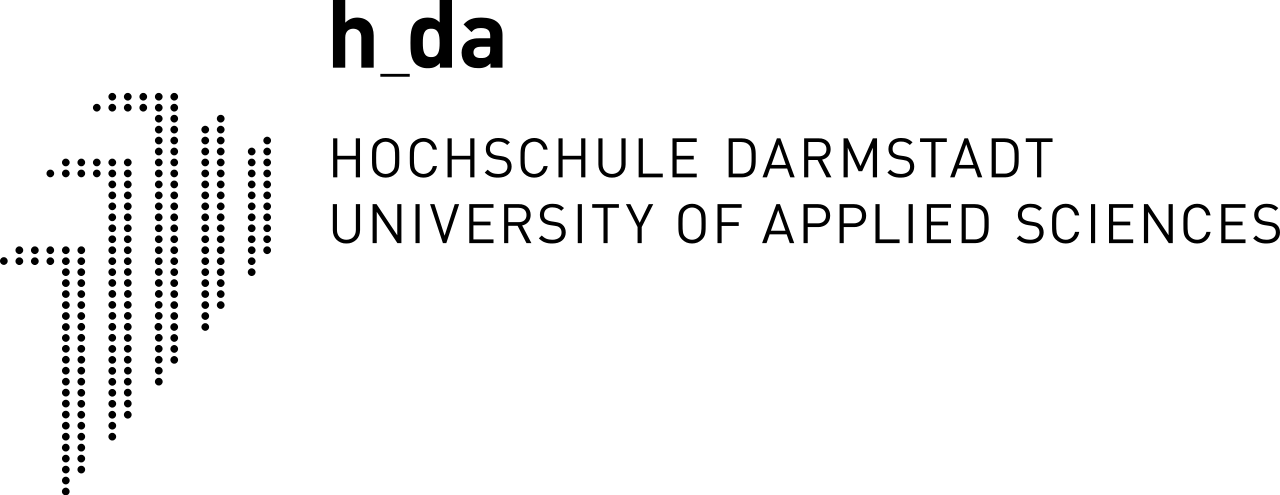
\includegraphics{res/Hda_logo}}
	\end{minipage}
\end{figure}

%----------------- INHALT ----------------- %

\begin{center}
	
	\LARGE Hochschule Darmstadt \\%\univname\\
	\Large \textsc{- Fachbereich Informatik -}\\ %\facname
	
	% Whitespace
	\vspace{60 pt}
	
	\LARGE \ttitle\\
	%\normalsize
	\vspace{20 pt}
	
	\large
	Abschlussarbeit zur Erlangung des akademischen Grades \degreename
	%Thesis~for~the~attainment~of~the~academic~degree\\
		
	vorgelegt von\\
	\vspace{8 pt}
	\begin{center}
		\huge
		John Doe\\ % no, using the author name from the variable does not work well :/
	\end{center}
	
	\today

	
	\vspace*{\fill}%
	\vfill
	
	\begin{tabular}[h]{p{4cm}l l}
		Referent: & \supname\\
		Korreferent: & \examname\\
	\end{tabular}
	

	
\end{center}
\end{titlepage}

%----------------------------------------------------------------------------------------
%	ABSTRACT PAGES
%----------------------------------------------------------------------------------------

\chapter*{Abstract (Deutsch)}
% !TeX spellcheck = de_DE
\par\vspace{10pt} % hier gib's noch ein bisschen Platz zur Not ;)

	
\enlargethispage{1pt} % ;) und hier nochmal

%%%%
% Abstract: 1 Seite, darf technisch sein, keine ausschweifende Erklärung möglich/nötig
%
	

% Was genau ist das Problem, Warum ist das ein Problem (A,B)


\blindtext[2]


\chapter*{Abstract}
% !TeX spellcheck = en_US
\par\vspace{10pt} % hier gib's noch ein bisschen Platz zur Not ;)

This is analogous to the German Abstract.


%----------------------------------------------------------------------------------------
%	DECLARATION PAGE
%----------------------------------------------------------------------------------------
%\chapter*{Erklärung}


\begin{declaration}
%	\addchaptertocentry{\authorshipname}
	
	
	 \noindent Ich versichere hiermit, dass ich die vorliegende Arbeit selbständig verfasst und keine anderen als die im Literaturverzeichnis angegebenen Quellen benutzt habe.
	 Alle Stellen, die wörtlich oder sinngemäß aus veröffentlichten oder noch nicht veröffentlichten Quellen entnommen sind, sind als solche kenntlich gemacht.
	 Die Zeichnungen oder Abbildungen in dieser Arbeit sind von mir selbst erstellt worden oder mit einem entsprechenden Quellennachweis versehen.
	 Diese Arbeit ist in gleicher oder ähnlicher Form noch bei keiner anderen Prüfungsbehörde eingereicht worden.
	
	\hfill\\

	\noindent Darmstadt, den \today\\
	\noindent
	
	\begin{minipage}[t]{.35\textwidth}
		\hfill
	\end{minipage}
	\authorname: \dotfill\strut

\end{declaration}


\cleardoublepage

%----------------------------------------------------------------------------------------
%	QUOTATION PAGE
%----------------------------------------------------------------------------------------

%\vspace*{0.2\textheight}
%
%\noindent\enquote{\itshape Thanks to my solid academic training, today I can write hundreds of words on virtually any %topic without possessing a shred of information, which is how I got a good job in journalism.}\bigbreak
%
%\hfill Dave Barry

%%%%%%%%%%%%%%%%%%%%%%%%%%%%%%%%%%
% Auf maximal einer Seite ist eine Kurzfassung der Arbeit anzugeben. Diese muss insbesondere 
% die Motivation für die Arbeit und die zugrunde liegenden Fragestellungen, die gewählte Vorgehensweise und durchgeführten Aktivitäten sowie das Ergebnis der Arbeit enthalten.  
% Das Abstrakt wird im Internet veröffentlicht. 
%%%%%%%%%%%%%%%%%%%%%%%%%%%%%%%%

%----------------------------------------------------------------------------------------
%	LIST OF CONTENTS/FIGURES/TABLES PAGES
%----------------------------------------------------------------------------------------
\setcounter{tocdepth}{2} % set numbering for toc
\setcounter{secnumdepth}{2} % set numbering for sections
%schon 3 ist grenzwertig% 

{% print more compact
	\singlespacing
\tableofcontents % Prints the main table of contents

\listoffigures % Prints the list of figures

\lstlistoflistings % prints the list of listings

\listoftables % Prints the list of tables

\renewcommand*{\glsgroupskip}{\vspace{1.2\bigskipamount}}% less space between groups, achieving a more compact list
\printglossary	 % Prints the glossary

}
%----------------------------------------------------------------------------------------
%	DEDICATION
%----------------------------------------------------------------------------------------

%\dedicatory{For/Dedicated to/To my\ldots} 

%----------------------------------------------------------------------------------------
%	THESIS CONTENT - CHAPTERS
%----------------------------------------------------------------------------------------

\pagestyle{thesis} % Return the page headers back to the "thesis" style

% Include the chapters of the thesis as separate files from the Chapters folder
% Uncomment the lines as you write the chapters
\begin{acknowledgements}
Ich danke meinen Prüfern und Betreuern, Herrn Prof. Dr. Max Baum und Prof. Dr. Jane Example, für...

\end{acknowledgements}
\mainmatter % Begin arabic (1,2,3...) page numbering
% !TeX spellcheck = de_DE
\chapter{Einführung}

\begin{formal}
Benutze paragraphs wenn, wenn sections zu viel Trennung zu viel sind aber du eine Gliederung deutlich machen willst. 
\end{formal}

\paragraph{Einordnung}
\gls{E2E} E-Mail Verschlüsselung gewann spätestens mit den
Snowden-Leaks 2013 auch außerhalb der IT-Szene an Bedeutung. % Using gls to use glossaries

\paragraph{Notwendigkeit }
\cite{googleemailsectrends} zeigt, dass die Verbreitung der Transportverschlüsselung zwischen den E-Mail-Servern und zum Nutzer zunimmt.

\begin{formal}
	Nutzung von Fußnoten und Acrfull
\end{formal}
\acrfull{E2E}-verschlüsselt\footnote{Repräsentative Umfrage von Bitkom: 15\% der Nutzer verschlüsselten in 2015 E-Mails teilweise \cite{bitkom-emailcrypto-langsam}}



\paragraph{Marktlücke}
\blindtext[1]

\paragraph{Arbeitsumfeld}
\begin{formal}
	Benutzung von \\emph für gewisse Eigennamen
\end{formal}
Verantwortlich für das Projekt ist die Abteilung \emph{Cloud Computing and Identity \& Privacy} des SIT.

Der Autor war von Februar bis Juni 2016 Teil des Teams und entwickelte dort die OpenPGP-Erweiterung, der dem Projekt zugrunde liegenden PKI.
\chapter{Problemstellung}

Liste mit Punkten die die Lösung erfüllen soll:

\blindenumerate[10]
% !TeX spellcheck = de_DE
\chapter{Grundlagen}

S/MIME ist standardisiertes Format zur Verschlüsselung von E-Mails und setzt X.509 Zertifikate ein. S/MIME und OpenPGP sind inkompatibel (Absatz vgl. \cite[S. 667f]{book:kryptoschmeh}).


\vref{fig:alice-bob-mallory} zeigt die beschriebenen drei bzw. vier Akteure der Kommunikation.

\begin{minipage}[c]{\textwidth}
	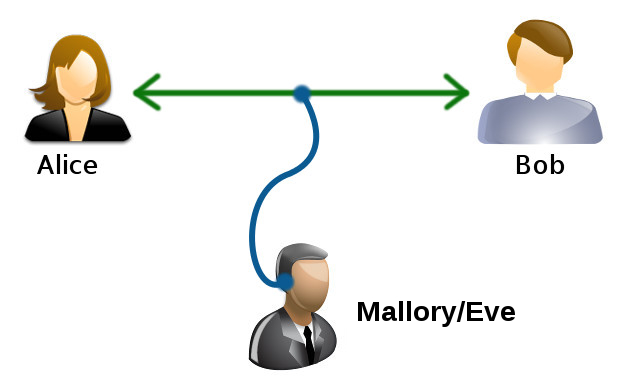
\includegraphics{res/Alice-bob-eve}
	\figcaption[Vorstellung von Alice, Bob und Mallory/Eve]{\mbox{Vorstellung von Alice, Bob und Eve}\\
		\footnotesize{Quelle: Ursprünglich von Didia (Own work) [CC BY-SA 4.0 (http://creativecommons.org/licenses/by-sa/4.0)], via Wikimedia Commons mit Änderung des Bezeichnung Mallory \cite{alicebobeve}}}
	\label{fig:alice-bob-mallory}
\end{minipage}


\section{OpenPGP}\label{openpgp}
\begin{formal}
	Cite mit Seitenangabe
\end{formal}
Es ist eines der am weitesten verbreiteten Werkzeuge zur E-Mail- und Dateiverschlüsselung~(\cite[S. 995]{book:cyclocryptosec}).

\begin{formal}
	Cite eines RFC
\end{formal}
1998 standardisierte die OpenPGP Working Group PGP bei der \gls{IETF} als "`OpenPGP Message Format"' in \cite{rfc4880}.

\begin{formal}
	vref,  smartref und autoref im Vergleich
\end{formal}

\textbf{\vref{loesung}}\\ 
\textbf{\smartref{loesung}}\\
\autoref{loesung}


\begin{formal}
	cite mit mehreren Quellen 
\end{formal}
\cite{heise-10jahrepgp, heise-gpgsupport, gpg-nytfounding, license-gpg})


\begin{formal}
	benutzung von verb
\end{formal}
In der vorliegenden Arbeit wird diese Software für Untersuchungen und zu Demonstationszwecken in den Versionen \verb|gpg 1.4.18| bzw. \verb|gpg2 2.0.28| verwendet



\begin{formal}
	Eine Referenz auf eine Zeile in einem Listing
\end{formal}
Die verwendeten Subpaket-Klassen beschränken sich lediglich auf 2 (Datum) und 29 (Grund des Widerrufs) in Zeile \ref{code:hashed-subpkt-2}f.

\begin{minipage}[t]{\textwidth}
	\begin{lstlisting}[language=bash,label={lst:pgp-packet},deletekeywords={test},caption={Ein PGP-Paket}]
:signature packet: algo 1, keyid 959FEB541D9FCFE5
version 4, created 1462880534, md5len 0, sigclass 0x30
digest algo 2, begin of digest b3 50
hashed subpkt 2 len 4 (sig created 2016-05-10)(*\label{code:hashed-subpkt-2}*)
hashed subpkt 29 len 15 (revocation reason 0x00 (this is a test))
subpkt 16 len 8 (issuer key ID 959FEB541D9FCFE5)
data: [2046 bits]
	\end{lstlisting}
\end{minipage}


\begin{formal}
	Eine in der Breite beschränkte Grafik (0.8)
\end{formal}

\begin{center}
\begin{minipage}[c]{0.8\textwidth}
	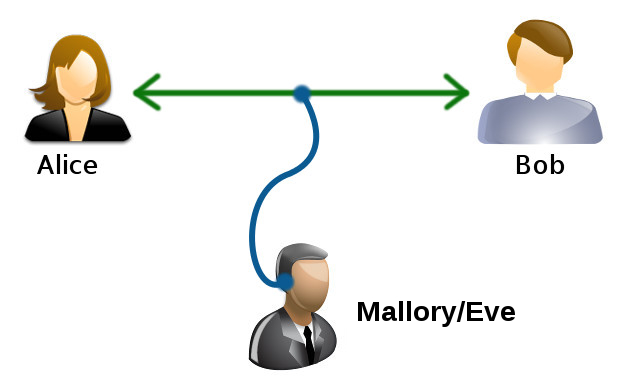
\includegraphics{res/Alice-bob-eve}
  \figcaption[Vorstellung von Alice, Bob und Mallory/Eve]{\mbox{Vorstellung von Alice, Bob und Eve}\\
	\footnotesize{Quelle: Ursprünglich von Didia (Own work) [CC BY-SA 4.0 (http://creativecommons.org/licenses/by-sa/4.0)], via Wikimedia Commons mit Änderung des Bezeichnung Mallory \cite{alicebobeve}}}
	\label{alicebob-2}
\end{minipage}
\end{center}


\begin{formal}
	Eine in der Höhe beschränkte Grafik (0.6); \textbf{Zeigen wie man subscripts in Captions unterbringt}
\end{formal}
\begin{figure}[h!]
	\centering
	\Oldincludegraphics[height=0.60\textheight]{res/Alice-bob-eve}
     \caption[Subscript in caption]{Subscript test \mbox{$Variable_{\textnormal{subscript}}$}\\
	\footnotesize{Quelle: Ursprünglich von Didia (Own work) [CC BY-SA 4.0 (http://creativecommons.org/licenses/by-sa/4.0)], via Wikimedia Commons mit Änderung des Bezeichnung Mallory \cite{alicebobeve}}}
	\label{key-upload-flowchart-section}
\end{figure}
\clearpage

\begin{formal}
	Eingerückter Text
\end{formal}

\begin{adjustwidth}{1em}{0em}

% Ja, das darf kein Paragraph sein, weil sonst die EInrückung nicht funktioniert
\keyword{1. Sitzungs-ID} 
Lorem ipsum dolor sit amet

\paragraph{2. Authentifizierung}
Lorem ipsum dolor sit amet

\paragraph{3. Verifikation}
Lorem ipsum dolor sit amet

\end{adjustwidth}


Ein Beispielaufruf des Uploads zeigt \vref{lst:ra-rest-cert-demo}.

\begin{formal}
	Inlining von Latex-Kommandos in Listings (z.B. zum Fett-drucken) (escapeinside)
\end{formal}
\begin{minipage}[t]{\textwidth}
	\begin{lstlisting}[label={lst:ra-rest-cert-demo},caption={Beispielanfrage zum Upload eines Keys},escapeinside={(\%}{\%)}]
(%\textbf{POST}%) (%\url{/certs/?pid=flJvlYAH...CKQZusIT&cert_type=encr}%) HTTP/1.1
[...]
(%\fbox{--01ead4a5-7a67-4703-ad02-589886e00923}%)
[...]
--01ead4a5-7a67-4703-ad02-589886e00923
	\end{lstlisting}
\end{minipage}
% !TeX spellcheck = de_DE

\chapter{Arbeitstitel-oder -thema (Lösung)}\label{loesung}
In diesem Kapitel wird die eigene Arbeit beschrieben, ein Konzept, Implementierung, Messergebnisse oder ähnliches.

\begin{formal}
	"`Sonderzeichen"' im Math-mode:\\
	$L\ddot{a}nge_{signatur} <= N$
\end{formal}



\begin{formal}
	Zentrieren eines Texts
\end{formal}
Eine typische UID sieht wie folgt aus:
\begin{center}
	\verb|Max Mustermann (beruflich) <mm@example.com>|
\end{center}


\begin{formal}
	Eine einfache Tabelle mit hervorgehobenen Boxen
\end{formal}
\begin{minipage}{\textwidth}
	\captionof{table}{Akzeptierte Reihenfolgen der Namensbestandteile einer UID}\label{accepted-namecombinations}
	\begin{tabular}{|l|c|l|l|c|}
		\toprule
		& &&& \textbf{Beispiel} \\
		\midrule
			\textbf{1} & \quickbox{Titel} &  \quickbox{Vornamen} &  \quickbox{Nachnamen}& Dr. Max Baum\\	
		\hline
			\textbf{2} & \quickbox{Titel} &  \quickbox{Nachnamen} &  \quickbox{Vornamen} &Dr. h. c. Ban Ki-moon\\		
		\hline
				\textbf{3} & & \quickbox{Vornamen} & \quickbox{Nachnamen}&Max Baum\\
		\hline
				\textbf{4} &  & \quickbox{Nachnamen} & \quickbox{Vornamen}&Ban Ki-moon\\
		\hline
				\textbf{5} &  & \quickbox{Nachnamen}\quickbox{,} & \quickbox{Vornamen}&Baum, Max \\
		\bottomrule
	\end{tabular}
\end{minipage}



\subsubsection{Kryptographische- und Sicherheits-Eigenschaften}

\begin{formal}
	Wörtliches Zitieren, zweisprachig
\end{formal}
\begin{quotation}
"`OpenPGP implementations MUST create keys with version 4 format. V3 keys are deprecated;"'~\cite[S.40]{rfc4880}\\
Deutsch:~\emph{OpenPGP Implementierungen müssen [zwingend] Schlüssel im Format der Version 4 erzeugen. Schlüssel der Version 3 sind veraltet;}
\end{quotation}



\begin{formal}
	Eine Description, genutzt zum Auflisten einer key-value Liste mit hervorgehobenem key 
\end{formal}
\begin{description}
	\item[OK]\hfill\\\verb|Prof. Dr. Frank Emil Schuster <fes@example.com>|
	\item[OK] Kein Titel\\\verb|Frank Emil Schuster <fes@example.com>|
	\item[Fehler] Unvollständiger Vorname\\\verb|Prof. Dr. Frank Schuster <fes@example.com>|
	\item[Fehler] Falsche E-Mail-Adresse\\\verb|Prof. Dr. Frank Emil Schuster <NOBODY@example.com>|
	\item[OK] Kommentare werden gefiltert\\\verb|(foo)Frank Emil Schu()ster (foo) <fes@exampl(foo)e.com>|
\end{description}

\begin{formal}
	Eine Description, mit minimierten Zeilenzwischenräumen
\end{formal}
\begin{description}[noitemsep]
	\item[$\approx$ 3s] Authentifikation und Stellung des Zertifizierungsauftrags
	\item[$\approx$ 2s bis 48s] Warten auf CA und XML-Austausch
	\item[$\approx$ 300ms] Herunterladen des Zertifikats und Senden eines Sperrauftrags
\end{description}



\clearpage
\begin{formal}
	Eine Komplexe, mehrzeilige Tabelle
\end{formal}
\begin{minipage}{\textwidth}
	%	\renewcommand{\arraystretch}{1.3}
	\captionof{table}{Überblick über Optionen der Publikation von Zertifikatsdaten} \label{publikationsfaelle} 
	\begin{tabular}{|l|c|c|c|}
		\hline
		\multirow{2}{*}{\textbf{Option}} & \multirow{2}{*}{\textbf{Verteilung}} & \multirow{2}{*}{\addstackgap{\shortstack{\textbf{Umfang} \\ \textbf{veröffentlichter Daten}}}}\footnote{Hervorgehobene Box steht für \quickbox{OpenPGP-Paket}} & \multirow{2}{*}{\textbf{Auffindbarkeit}}\\
		&&&\\
		\hline
		1 & Manuell & Keine & Keine\footnote{solange keine Sperrung vorliegt} \\
		\hline
		\multirow{3}{*}{2} & \multirow{3}{*}{Keyserver} & \multirow{3}{*}{\addstackgap{\shortstack{ \quickbox{Public-Key-Material}\\ \quickbox{(PGPCA-)Signatur}}}} & \multirow{3}{*}{per Key-ID\footnote{keine Preisgabe von personenbezogenen Daten}} \\
		&&&\\
		&&&\\
		\hline
		\multirow{3}{*}{3} & \multirow{3}{*}{Keyserver} & \multirow{3}{*}{\addstackgap{\shortstack{\quickbox{Public-Key-Material} \\ \quickbox{User-ID + Selbst-Signatur} \\ \quickbox{(PGPCA-)Signatur}}}} & per Key-ID, \\
		&&&E-Mail Adresse,\\
		&&&Namen\\
		&&&\\
		\hline
	\end{tabular}
\end{minipage}

\chapter{Implementierung}\label{implementierung-abgrenzung}
Was wurde vom Konzept implementiert, was fehlt noch, was ist unvollständig?

\keyword{Vollständig}
\blindtext

\keyword{Unvollständig}
\blindtext

\keyword{Ausstehend}
\blindtext
% !TeX spellcheck = de_DE
\chapter{Auswertung}

\section{Überprüfung der Anforderungserfüllung}
\begin{enumerate}
	\item \textbf{Anforderung 1}\\
		Anforderung 1 wurde erfüllt, weil... So wurde es gelöst (kurz)

	\item \textbf{Anforderung 2}\\
		Anforderung 2 wurde erfüllt, weil... So wurde es gelöst (kurz)
		
\end{enumerate}
%\include{Chapters/Verwandte-Arbeiten}
% !TeX spellcheck = de_DE
\chapter{Zusammenfassung}
	
Was leistet die Lösung, was wurde gelöst, welche Kritik gibt es, was hat diese Arbeit erreicht für die Forschung und andere Bereiche? Welche Erkenntnisse gewann der/dir Autor*in beim Schreiben?
\chapter{Ausblick}

Was wird mit dem Thema weiter passieren, sind Trends abzusehen, wird die Relevanz des Themas bleiben?

\section{Weiterentwicklung }\label{weiterentwicklung}
Welche Weiterentwicklung wird/muss passieren?

\section{Forschung}

Welche Forschungsbereiche/-Fragen wurden entdeckt, könnten in Zukunft bearbeitet werden?



%----------------------------------------------------------------------------	------------
%	THESIS CONTENT - APPENDICES
%----------------------------------------------------------------------------------------


% Include the appendices of the thesis as separate files from the Appendices folder	
% Uncomment the lines as you write the Appendices
\appendix % all following chapters are appendices


\chapter{Listings}
\section{Programmablauf Hello World}
\blindtext[1]

\begin{minipage}[t]{\textwidth}
	\begin{lstlisting}[language=Java,style=eclipse-java,label={lst:helloworld-class},caption={Code Fragment of Hello World Class}]
/**
* The HelloWorldApp class implements an application that
* simply prints "Hello World!" to standard output.
*/
class HelloWorldApp {
	public static void main(String[] args) {
	System.out.println("Hello World!"); // Display the string.
	}
}
	\end{lstlisting}
\end{minipage}
%\include{Appendices/AppendixB}
%\include{Appendices/AppendixC}

%----------------------------------------------------------------------------------------
%	BIBLIOGRAPHY
%----------------------------------------------------------------------------------------

\printbibliography[heading=bibintoc]

%----------------------------------------------------------------------------------------

\end{document}  

% TODO
% Consistency in language task + Ausbau der Definition
% * Zertifizierung ist der Vorgang
% * zertifikat ist das was beim vorgang rauskommt
% * Signatur ist ein teil des zertifikats (keine Metadaten)